% Created 2020-02-09 Sun 20:51
% Intended LaTeX compiler: pdflatex
\documentclass[11pt]{article}
\usepackage[utf8]{inputenc}
\usepackage[T1]{fontenc}
\usepackage{graphicx}
\usepackage{grffile}
\usepackage{longtable}
\usepackage{wrapfig}
\usepackage{rotating}
\usepackage[normalem]{ulem}
\usepackage{amsmath}
\usepackage{textcomp}
\usepackage{amssymb}
\usepackage{capt-of}
\usepackage{hyperref}
\usepackage[pdf]{graphviz}
\usepackage{natbib}
\usepackage{multirow}
\usepackage{array}
\usepackage{chngpage}
\hypersetup{colorlinks=true, linkcolor=black, citecolor=black, filecolor=black, urlcolor=black}
\author{Marcus Lewis}
\date{\today}
\title{Achieving sparse connectivity via backprop-trained permanences}
\hypersetup{
 pdfauthor={Marcus Lewis},
 pdftitle={Achieving sparse connectivity via backprop-trained permanences},
 pdfkeywords={},
 pdfsubject={},
 pdfcreator={Emacs 26.3 (Org mode 9.1.9)}, 
 pdflang={English}}
\begin{document}

\maketitle
\frenchspacing

\section{Summary}
\label{sec:orgeabd57d}

In the past, we have modeled synapses using \emph{permanences}. Typically, a permanence is a scalar between 0 and 1. If a permanence is above a threshold, typically 0.5, the synapse exists; otherwise it doesn't. Each permanence is trained using Hebbian learning.

In this work, I show how the notion of synapse permanence fits into deep neural networks. There is one fundamental change: rather than using Hebbian learning, the permanences are trained using the backpropagated gradient.

This technique can be used for many tasks. For example, it can be used to train networks with binary synapses \citep{courbariaux2015binaryconnect} and binary activations \citep{courbariaux2016binarized}. In this work, I add permanences to networks that already have synaptic weights, and I use the permanences as a synapse pruning/growth mechanism. By imposing a constant decay on each permanence, I train networks that optimize for both accuracy and weight sparsity. As expected, these dynamic sparse networks are sparser and more accurate than our static sparse networks \citep{ahmad2019dense}.

I include noise tolerance results, using the form of noise tolerance from \cite{ahmad2019dense}. This form of noise tolerance is influenced by many details of the training process. Sparse connectivity on its own does not provide a consistent noise tolerance benefit. Batch normalization provides an accuracy improvement but it reduces noise tolerance.

I suggest that this model can be understood as performing a form of averaging of the error gradient for each connection, pruning connections whose average falls below a certain threshold, and implementing this algorithm using permanences.


\section{Model}
\label{sec:orgbb0d4e2}

This model has two modes: \emph{deterministic} and \emph{stochastic}. In deterministic mode, permanences are thresholded at 0.5. In stochastic mode, each synapse has some probability of existing, and the permanence serves as this probability. The experiments in this paper use stochastic mode, but similar results can be achieved with deterministic mode if you combine it with some regularization strategy (for example, dropout).

\begin{figure}[htbp]
\centering
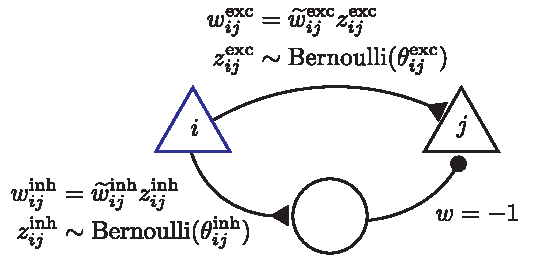
\includegraphics[width=4in]{./figures/model.pdf}
\caption{Every connection in this model. (Stochastic mode) \label{fig:model}}
\end{figure}

Every connection is modeled with two synapses: an inhibitory and an excitatory synapse (\textbf{Figure \ref{fig:model}}). Each synapse has two parameters: a weight \(\tilde{w}_{ij}\) and a permanence \(\theta_{ij}\). On each forward pass, the synapse's sampled weight \(w_{ij}\) is calculated by sampling a Bernoulli random variable with probability \(\theta_{ij}\), then multiplying the result with stored weight \(\tilde{w}_{ij}\).

Backpropagation can compute gradients for activation \(a_j\), weight \(w_{ij}\), and even the gate value \(z_{ij}\), but changing the permanence \(\theta_{ij}\) causes discrete rather than continuous changes to activations, so a different strategy is needed for training permanences. To enable backpropagation to propagate through the Bernoulli operation, I estimate the gradient of the \emph{expected} error or reward \(E\left[f\right]\) using the straight-through estimator \citep{bengio2013estimating} as follows:

$$
\frac{dE[f]}{d\theta_{ij}} \approx \frac{df}{dz_{ij}}
$$

The quantity \(df/dz_{ij}\) is calculated using basic rules of backpropagation:

$$
\frac{dE[f]}{d\theta_{ij}} \approx \frac{df}{da_j} * \tilde{w}_{ij} a_i
$$

This can be understood as estimating how changing the permanence changes the expected value of unit \(j\) (the \(\tilde{w}_{ij} a_i\) term on the right) and multiplying that with unit \(j\)'s gradient. Thus, when using basic gradient descent with learning rate \(\eta\), the permanence update is computed via:

$$
\Delta\theta_{ij} = -\eta * \left( \frac{df}{da_j} * \tilde{w}_{ij} * a_i \right)
$$

With Bernoulli gated synapses, this estimator can be shown to be unbiased (see Appendix). Surprisingly, in deterministic mode, this same update rule still works nicely, even though the rule was derived with the assumption that the permanence is a Bernoulli parameter (see Discussion).

I allow permanences to go outside the bounds \([0, 1]\). This enhances the network's ability to accumulate history and produces good results. When a permanence is outside these bounds, the unit behaves as if the permanence is at the bound.

To sparsify the network, I impose a constant decay on each permanence, adding a constant \(\lambda\) to its gradient. If I set this decay to always move the weight toward 0, it works well, but it often removes all synapses from entire units. Instead, I calculate each layer's mean number of synapses per unit, denoted \(\mu\), with a different \(\mu\) for every layer, and I set the decay to push each unit's number of synapses toward \(\mu/2\). This sparsifies the network without killing units. This decay is implemented similarly to an \(L_1\) regularization on the permanence, centered on \(\mu/2\). This can also be described as \(L_0\) regularization of the weights \citep{louizos2018learning}, paying a cost for the expected number of nonzero weights. I use the same constant for every layer; better results will be attainable by tuning different \(\lambda\) constants per layer.


\section{Results}
\label{sec:orgea40d05}

I trained this dynamic sparsity model on the Google Speech Commands (GSC) and MNIST datasets, and I measured the trained network's test accuracy and its number of nonzero weights.

\subsection{Compared to static sparsity, dynamic sparsity achieves higher accuracy with fewer weights.}
\label{sec:org3d43693}

There are two objectives: maximize the accuracy, minimize the number of weights. The model has a set of hyperparameters that can be tuned to prefer either objective. Thus, the model's performance is best understood by showing results for multiple optimal model configurations, using different definitions of \emph{optimal}. This set of solutions is known as the Pareto frontier. To find the Pareto frontier, I performed a set of Bayesian hyperparameter searches. For each search I used a different objective function that assigned different weights to the two underlying objectives (log-error and log-number-of-nonzero-weights).

Results for both datasets are shown in \textbf{Figure \ref{fig:gsc-mnist-main}}. Comparing to the result from \citep{ahmad2019dense} (shown as orange 'X' marks with label "HSD"), this model is able to achieve the same accuracy with fewer weights, or it can achieve higher accuracy with the same number of weights. Precise numbers for two of the GSC results are shown in \textbf{Table \ref{table:gsc-weights}} alongside results using the static sparsity model from \citep{ahmad2019dense} and a dense model. The permanence method can achieve similar accuracy with fewer weights (38,784 weights at accuracy \(\approx\)96.75\%, as opposed to 193,280), and it can achieve better accuracy with the same number of weights (97.13\%  with \(\approx\)190,000 weights, as opposed to 96.71\%). Similar results can be seen on MNIST (shown in Figure \ref{fig:gsc-mnist-main} but not the table). Again, the permanence method results in the same accuracy with fewer weights (25,710 weights at accuracy \(\approx\)99.16\%, as opposed to 173,880 weights) and better accuracy with the same number of weights (99.33\% with \(\approx\)160,000 weights, as opposed to 99.16\%).

\begin{figure}[htbp]
\centering
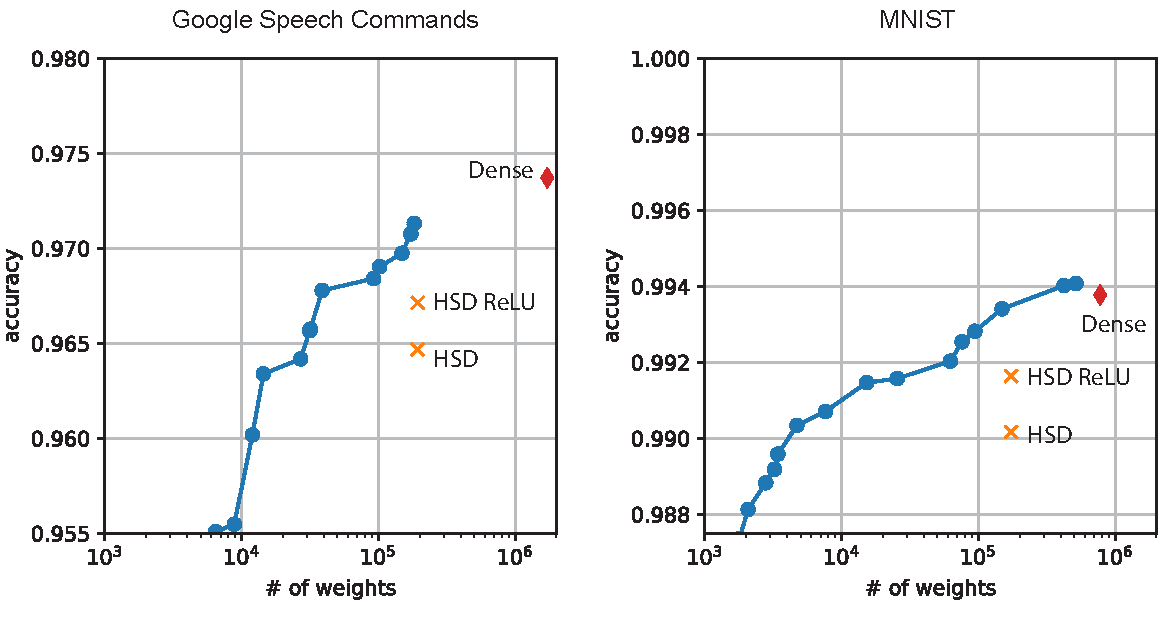
\includegraphics[width=5in]{./figures/gsc-mnist-main.pdf}
\caption{Accuracy and weight sparsity on two datasets. \label{fig:gsc-mnist-main}}
\end{figure}


\begin{table}
\begin{adjustwidth}{-1in}{-1in}
\begin{center}
\begin{tabular}{cc|ccccc}
\textit{\textbf{Weights}} & & Conv1 & Conv2 & FC1 & FC2 & \textbf{Total} \\
\hline

\multirow{3}{7.95em}{\textbf{Dense} \\ 97.37\% accuracy}
  & \textit{Percent}  & 100\% & 100\% & 100\% & 100\% & 100\% \\
  & \textit{Total}    & 1,600 & 102,400 & 1,600,000 & 12,000 & \textbf{1,716,000} \\
  & \textit{Per unit} & 25 & 1,600 & 1,600 & 1,000 & \\
    \hline
\multirow{3}{7.95em}{\textbf{Dynamic sparse} \\ 97.13\% accuracy}
  & \textit{Percent}  & 41\% & 22\% & 10\% & 13\% & 11\% \\
  & \textit{Total}    & 662 & 22,394 & 158,150 & 1,520 & \textbf{182,725} \\
  & \textit{Per unit} & 10 & 350 & 158 & 127 & \\
    \hline
\multirow{3}{7.95em}{\textbf{Dynamic sparse} \\ 96.78\% accuracy}
  & \textit{Percent}  & 30\% & 7\% & 2\% & 12\% & 2\% \\
  & \textit{Total}    & 482 & 7,321 & 29,570 & 1,410 & \textbf{38,784} \\
  & \textit{Per unit} & 8 & 114 & 30 & 118 & \\
    \hline
\multirow{3}{7.95em}{\textbf{Static sparse} \\ 96.71\% accuracy}
  & \textit{Percent}  & 50\% & 20\% & 10\% & 100\% & 11\% \\
  & \textit{Total}    & 800 & 20,480 & 160,000 & 12,000 & \textbf{193,280} \\
  & \textit{Per unit} & 12 & 320 & 160 & 1,000 & \\

\end{tabular}

\vspace{15}

\begin{tabular}{c|cccc >{\bf}c}
\textit{\textbf{Multiplies}} & Conv1 & Conv2 & FC1 & FC2 & Total \\
\hline

\multirow{2}{7.95em}{\textbf{Dense} \\ 97.37\% accuracy}
    & \multirow{2}{4em}{\raggedleft 1,254,400}
    & \multirow{2}{4.5em}{\raggedleft 10,240,000}
    & \multirow{2}{4em}{\raggedleft 1,600,000}
    & \multirow{2}{2.5em}{\raggedleft 12,000}
    & \multirow{2}{5em}{\raggedleft 13,106,400} \\
    \\
    \hline
\multirow{2}{7.95em}{\textbf{Dynamic sparse} \\ 97.13\% accuracy}
    & \multirow{2}{4em}{\raggedleft 518,851}
    & \multirow{2}{4.5em}{\raggedleft 2,239,420}
    & \multirow{2}{4em}{\raggedleft 158,150}
    & \multirow{2}{2.5em}{\raggedleft 1,520}
    & \multirow{2}{5em}{\raggedleft 2,917,941} \\
    \\
    \hline
\multirow{2}{7.95em}{\textbf{Dynamic sparse} \\ 96.78\% accuracy}
    & \multirow{2}{4em}{\raggedleft 378,202}
    & \multirow{2}{4.5em}{\raggedleft 732,080}
    & \multirow{2}{4em}{\raggedleft 29,570}
    & \multirow{2}{2.5em}{\raggedleft 1,410}
    & \multirow{2}{5em}{\raggedleft 1,141,262} \\
    \\
    \hline
\multirow{2}{7.95em}{\textbf{Static sparse} \\ 96.71\% accuracy}
    & \multirow{2}{4em}{\raggedleft 627,200}
    & \multirow{2}{4.5em}{\raggedleft 2,048,000}
    & \multirow{2}{4em}{\raggedleft 160,000}
    & \multirow{2}{2.5em}{\raggedleft 12,000}
    & \multirow{2}{5em}{\raggedleft 2,847,200} \\
    \\

\end{tabular}

\end{center}
\end{adjustwidth}
\caption{\textbf{Nonzero weights and multiplies in each layer.} Two dynamic sparse results are included, one with a similar density and one with a similar accuracy to that of the static sparse model. In both cases the dynamic sparse model excels on the other dimension. In the multiplies table, a multiply is defined as any multiplication in which the weight is nonzero, and the table shows the number of multiplies in a single inference. FC: "Fully connected layer", Conv: "Convolutional layer". For the dynamic sparse model, the "Per unit" numbers denote the mean number of weights per unit. For static sparse, it is the exact number. The static sparse network is the HSD ReLU point from Figure \ref{fig:gsc-mnist-main}. Dataset: GSC.}
\label{table:gsc-weights}
\end{table}


\subsection{Dynamic sparsity does not by itself consistently improve noise tolerance.}
\label{sec:org708be52}

In \citep{ahmad2019dense}, we tested a third objective: a specific type of noise tolerance. We added white noise to the test set, but we never added it to the training set. We evaluated models on whether they get resilience to this type of noise for free, i.e. without needing to train on it and without considering noise tolerance while tuning the hyperparameters. \textbf{Figure \ref{fig:gsc-mnist-noise}} shows the noise tolerance of the networks from Figure \ref{fig:gsc-mnist-main}. I have not added sparse activation yet, so this is an exploration of the impact of sparse connectivity alone on noise tolerance. I find that sparsely connected networks are not clearly more noise tolerant or less noise tolerant than dense networks. As I change the model's hyperparameters to increase sparsity, the noise tolerance decreases; it seems to simply go hand-in-hand with test accuracy.

Observing the change from "HSD ReLU" to "HSD" in figures \ref{fig:gsc-mnist-main} and \ref{fig:gsc-mnist-noise}, it is likely that adding sparse activation to this model will increase noise tolerance, though it may reduce accuracy.

\begin{figure}[htbp]
\centering
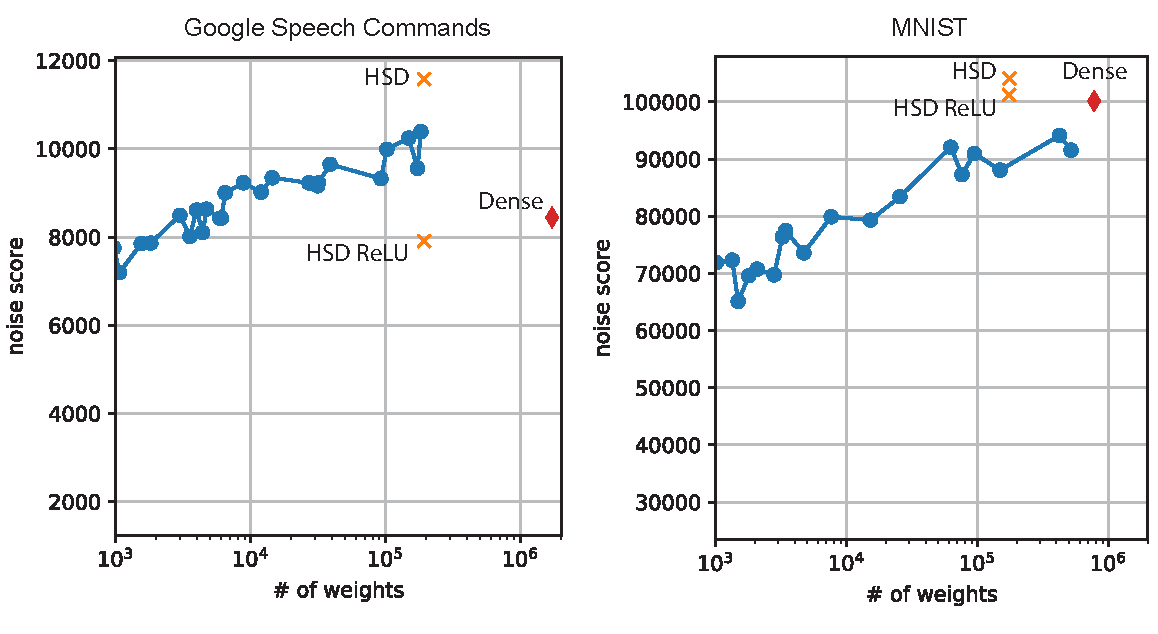
\includegraphics[width=5in]{./figures/gsc-mnist-noise.pdf}
\caption{Noise tolerance on two datasets (higher is better) \label{fig:gsc-mnist-noise}}
\end{figure}


\subsection{Batch normalization improves accuracy but reduces noise tolerance, at least on MNIST.}
\label{sec:org299a864}

In these experiments, following the lead of \citep{ahmad2019dense},  the MNIST network does not use batch normalization, while the GSC network does. I experimented with adding batch normalization to the MNIST network, and the results are shown in \textbf{Figure \ref{fig:mnist-batchnorm}}.

\begin{figure}[htbp]
\centering
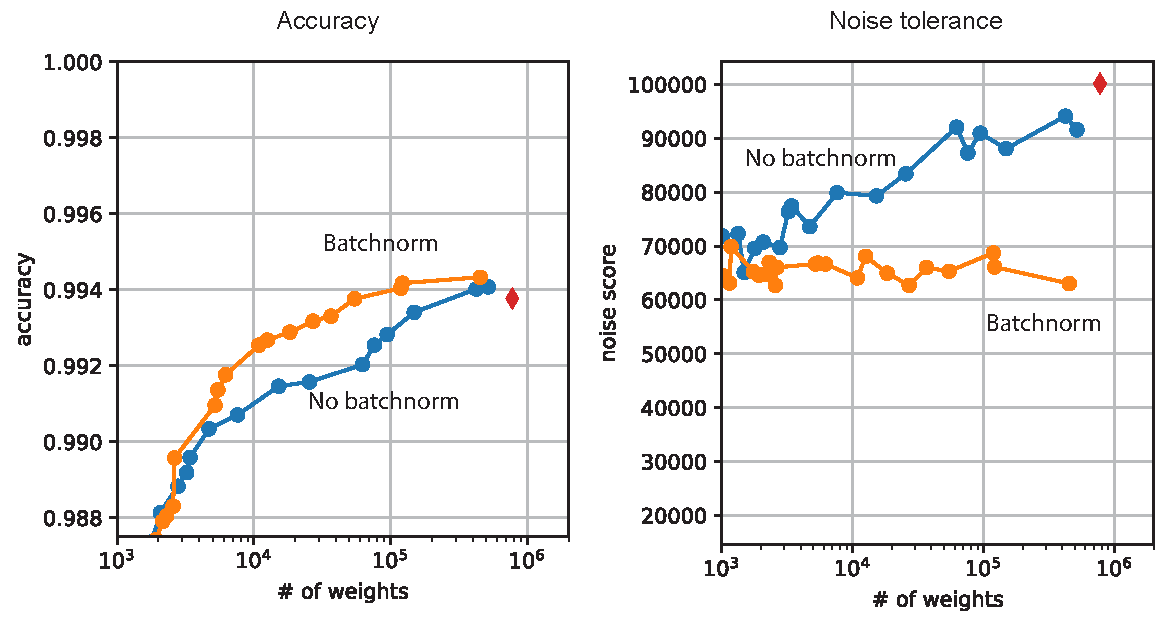
\includegraphics[width=5in]{./figures/mnist-batchnorm.pdf}
\caption{MNIST performance change with batch normalization \label{fig:mnist-batchnorm}}
\end{figure}

Batch normalization improves the network's accuracy while greatly reducing its noise tolerance. One possible explanation for this phenomenon is as follows. Batch normalization is specifically designed to keep the network's statistics from varying wildly during training. Without batch normalization, the network needs to bear more of the burden of handling changes in activation statistics. During test time, batch normalization is no longer capable of adapting to the new statistics, so a network that was trained without batch normalization tends to be more equipped to deal with the noise.

On the GSC dataset I performed two exploratory experiments. First, I tried training without batch normalization, but the network never achieved better-than-random test performance, so a new hyperparameter search is necessary. I did not go further, so this experiment was inconclusive on whether batch normalization affects GSC noise tolerance similarly to MNIST noise tolerance. Second, I changed the batch normalization so that it recomputes statistics at test time (by disabling "track\_running\_stats") and it caused the noise tolerance to dramatically improve, reaching noise scores around 14,500 on GSC. This strategy requires batching the test examples, so it would not work in a streaming inference system, though it does suggest that a streaming inference system could improve its noise tolerance by slowly updating its batch normalization "running stats" over time.

All of these noise tolerance results suggest that this type of noise can be understood as perturbing the activation statistics of the network. If the network has a mechanism for dealing with perturbed activation statistics, it will be better at handling this type of noise.

\section{Discussion}
\label{sec:orgde2512d}

Here I have presented a form of dense-to-sparse training. Even when the network is sparse, during training it is still considering how to change the permanence for every potential synapse on each active cell, so from the learning perspective the network is still fully dense. Permanences could be combined with another technique, for example periodic updating of an otherwise static structure, to provide fully sparse training.

I optimized for reducing the number of weights in the model, but arguably it would be better to reduce the number of multiplies. As seen in Table \ref{table:gsc-weights}, most of the weights are in the fully connected layers, while most of the multiplies occur in the convolutional layers. When optimizing for number-of-multiplies, there is a much larger incentive to remove weights from the convolutional layers than from fully connected layers. Because I used a single permanence decay rate for all layers, it did not make much difference whether I optimized for number-of-weights or number-of-multiplies. Better results will be possible by choosing different decay rates for each layer, but it may be best to switch to optimizing number-of-multiplies first.

The technique could also be used to train networks with binary weights, where all learning is in the structure, similar to most of our non-deep-learning models. This has already been shown in \citep{courbariaux2016binarized}, though that work defined binary as -1 or 1, not 0 or 1, so it does not have a notion of sparse connectivity. To my knowledge, nobody has used this technique to train sparse fully binarized networks. A binarized version of the model in this paper would have weights that are -1, 0, or 1, so some would argue that this would actually be a ternary network, but dedicating different neurons to excitation and inhibition (as in Figure \ref{fig:model}) would make it binary from a biological standpoint.


\subsection{What is this model fundamentally doing?}
\label{sec:orge5060c3}

I began this project with the narrative that this model would use stochastic synapses to explore which synapses ought to exist. I derived the update rule based on this narrative. So I was surprised to see that this update rule works even when the synapses are not stochastic, when instead the permanence is thresholded at 0.5. Others have found the same; \citep{courbariaux2015binaryconnect} and \citep{courbariaux2016binarized} tried both the stochastic and the deterministic version, and they found that the deterministic version worked sufficiently well (and is faster).

The fact that this works with deterministic synapses turns the narrative on its head. In \textbf{Figure \ref{fig:narrative}} I depict a new narrative. At the core, this algorithm is checking whether each synapse's mean gradient is above some threshold. The permanence decay is pushing the permanence in one direction, while the gradient is potentially pushing in the other direction. If the gradient is larger on average, the synapse will survive. If it is smaller, it will be pruned.

\begin{figure}[htbp]
\centering
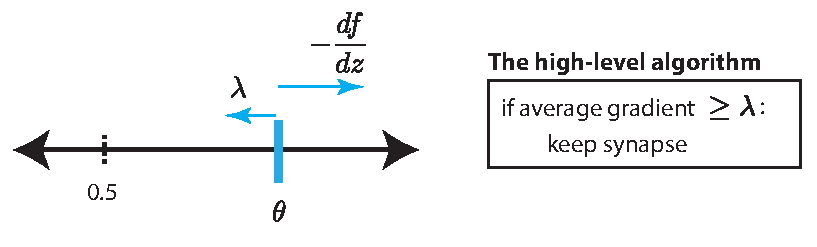
\includegraphics[width=.9\linewidth]{./figures/effective-algorithm.pdf}
\caption{An explanation that incorporates deterministic mode \label{fig:narrative}}
\end{figure}

Thus, this whole permanence system may just be a roundabout way of tracking whether the average gradient is above a threshold.

Seen in this light, this technique is philosophically similar to pruning weights by magnitude, since the weight is also formed by an accumulated gradient that is often pushing against a decay. One potential benefit of this alternative strategy is that it decouples the task of finding the optimal value of a weight from the task of deciding how much benefit that connection is providing.


\bibliographystyle{unsrt}
\bibliography{bib-backprop-permanences}


\newpage


\section{Appendix}
\label{sec:org155eddc}


\subsection{The network}
\label{sec:org702a269}
The source code for this model and these experiments can be found at \linebreak \url{https://github.com/numenta/nupic.research/tree/master/projects/backprop\_structure}

I used the same networks as \citep{ahmad2019dense}. The network used for the Google Speech Commands is shown in Figure \ref{fig:architecture-gsc}. The MNIST network was similar, just with different numbers of cells in each layer; it used 32 channels in the first Conv layer rather than 64, and 700 units in the fully connected layer rather than 1000.

\begin{figure}[htbp]
\centering
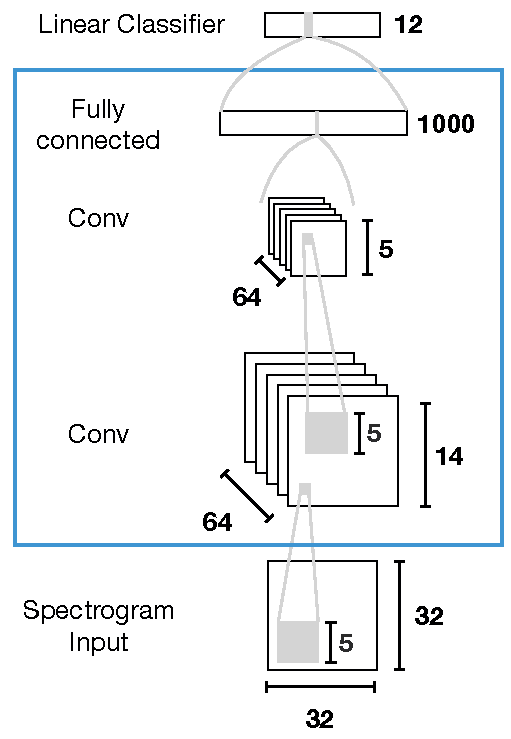
\includegraphics[width=3in]{./figures/architecture-gsc.pdf}
\caption{Google Speech Commands network \label{fig:architecture-gsc}}
\end{figure}




\subsection{Deriving the permanence update rule}
\label{sec:orgc3f0339}

In stochastic mode, the permanence update rule can be understood as performing gradient descent on the expected loss via Monte Carlo methods.

Recall that \(\theta_{ij}\) denotes the permanence of the synapse between unit \(i\) and unit \(j\), and \(\z{ij}\) denotes the binary value of its associated Bernoulli random variable, also known as a \emph{gate}.  At any point in time, each \(\theta_{ij}\) has a discrete impact on the reward or error \(f\), so \(f\) is not differentiable w.r.t. \(\theta_{ij}\). However, \(\theta_{ij}\) has a smooth effect on the \emph{expected} reward or error. Computing this exact value requires an intractable summation over all possible \(z\) vectors, but it can be estimated using Monte Carlo methods. We sample \(L\) different sets of gate values, compute the gradient for each, and approximate the actual gradient to be the mean of these sampled gradients. Let \(z_{-ij}\) denote all of the gates excluding \(z_{ij}\). z\(_{\text{-ij}}^{\text{(l)}}\) denotes the \(l\text{th}\) random sample of distribution \(p(z_{-ij} |\theta_{-ij})\).

\begin{align*}
\frac{d}{d\theta_{ij}}E[f] &=
\frac{d}{d\theta_{ij}}\sum_{\bm{z}}{p(\bm{z} | \bm{\theta}) f(\bm{z})} \\
&=
\frac{d}{d\theta_{ij}}\sum_{\bm{z_{-ij}}}{p(\bm{z_{-ij}} | \bm{\theta_{-ij})} \sum_{z_{ij}}{p(z_{ij} | \theta_{ij}) f(\bm{z_{-ij}}, z_{ij})}} \\
&\approx
\frac{d}{d\theta_{ij}}\frac{1}{L}\sum_{l=1}^L{\sum_{z_{ij}}{p(z_{ij} | \theta_{ij}) f(\bm{z_{-ij}^{(l)}}, z_{ij})}}
\end{align*}

Set \(L\) to \(1\) and rewrite the formula, shortening the \(f()\) notation so that it implicitly includes \(z_{-ij}^{(1)}\), giving us

$$
\frac{d}{d\theta_{ij}}E[f] \approx \frac{d}{d\theta_{ij}}\sum_{z_{ij}}{p(z_{ij} | \theta_{ij})f(z_{ij})}
$$

This estimate is much more tractable to compute, but it is still expensive and nonlocal. Although we've removed the combinatorial problem, for each permanence we would have to separately recompute the global function \(f\) for both possible values of its \(z\):

\begin{align*}
\frac{d}{d\theta_{ij}}\sum_{z_{ij}}{p(z_{ij} | \theta_{ij})f(z_{ij})} &=
 \frac{d}{d\theta_{ij}}\left[
(1 - \theta_{ij})f(z_{ij}=0) +
\theta_{ij}f(z_{ij}=1)
\right]
\\
&= \frac{d}{d\theta_{ij}}\left[
\Big(f(z_{ij}=1) - f(z_{ij}=0)\Big)*\theta_{ij} + f(z_{ij}=0)
\right]
\\
&= f(z_{ij}=1) - f(z_{ij}=0)
\end{align*}

Rather than recomputing \(f()\), the difference between its two values can be locally estimated by using the gate's gradient:

$$
\approx \frac{df}{dz_{ij}}
= \frac{df}{dw_{ij}} \frac{dw_{ij}}{dz_{ij}}  = \frac{df}{dw_{ij}} \widetilde{w}_{ij}
$$

To see this, note that at any particular time, one of the values \(f(z_{ij}=0)\) or \(f(z_{ij}=1)\) is known, and the other can be approximated using a first-order Taylor approximation, given that we know \(df/dz_{ij}\), which is obtained using basic backpropagation. In either scenario, substituting the approximation for \(f(z_{ij}=1)\) or \(f(z_{ij}=0)\) respectively, the result is \(df/dz_{ij}\).

This estimator can also be used for propagating gradients across binary unit activations. For this use case, the estimator is biased; although the thresholded sum of a set of Bernoulli random variables \(x_i\) is itself a Bernoulli random variable \(y\), the probability \(\theta_y\) won't change at a constant rate as the \$\(\theta_{\text{i}}\)\$s change, even when they change all together. Nonetheless, the strategy works empirically [2], so we set \(dE[f]/d\tilde{a}_j \approx df/da_j\) where \(\tilde{a}_j\) and \(a_j\) denote the unit's activity before and after the nonlinearity, and \(df/da_j\) denotes the backpropagating gradient.
\end{document}
